% Straight up stealing preamble from Eli Holmes 
%%%%%%%%%%%%%%%%%%%%%%%%%%%%%%%%%%%%%%START PREAMBLE THAT IS THE SAME FOR ALL EXAMPLES
\documentclass{article}

%Required: You must have these
\usepackage{Sweave}
\usepackage{graphicx}
\usepackage{tabularx}
\usepackage{hyperref}
\usepackage{natbib}
\usepackage{gensymb}
\usepackage{authblk}
\renewcommand{\baselinestretch}{1.8}
\usepackage{lineno}
%\usepackage[backend=bibtex]{biblatex}
%Strongly recommended
 %put your figures in one place
 
%you'll want these for pretty captioning
\usepackage[small]{caption}

\setkeys{Gin}{width=0.8\textwidth} %make the figs 50 perc textwidth
\setlength{\captionmargin}{30pt}
\setlength{\abovecaptionskip}{10pt}
\setlength{\belowcaptionskip}{10pt}
% manual for caption http://www.dd.chalmers.se/latex/Docs/PDF/caption.pdf

%Optional: I like to muck with my margins and spacing in ways that LaTeX frowns on
%Here's how to do that
 \topmargin -2cm     
 \oddsidemargin -0.04cm   
 \evensidemargin -0.04cm  % same as oddsidemargin but for left-hand pages
 \textwidth 16.59cm
 \textheight 22.94cm 
 %\pagestyle{empty}       % Uncomment if don't want page numbers
 \parskip 7.2pt           % sets spacing between paragraphs
 %\renewcommand{\baselinestretch}{1.5} 	% Uncomment for 1.5 spacing between lines
\parindent 0pt% sets leading space for paragraphs
\usepackage{setspace}
%\doublespacing

%Optional: I like fancy headers
\usepackage{fancyhdr}
\pagestyle{fancy}
\fancyhead[LO]{How do climate change experiments actually change climate?}
\fancyhead[RO]{2017}
 
%%%%%%%%%%%%%%%%%%%%%%%%%%%%%%%%%%%%%%END PREAMBLE THAT IS THE SAME FOR ALL EXAMPLES

%Start of the document
\begin{document}

% \SweaveOpts{concordance=TRUE}
\bibliographystyle{/Users/aileneettinger/citations/Bibtex/styles/ecol_let.bst}
\setkeys{Gin}{width=\textwidth}

\title{How do climate change experiments actually change climate?} 
%The title page must also contain full name(s), affiliation(s) and e-mail address(es) of all author(s)

\author[1,2,a]{A.K. Ettinger}

\author[3,b]{I. Chuine}

\author[4,5,c]{B.I. Cook}

\author[6,d]{J.S. Dukes}

\author[7,e]{A.M. Ellison}

\author[8,f]{M.R. Johnston}

\author[9,g]{A.M. Panetta}


\author[10,h]{C.R. Rollinson}

\author[11,12,i]{Y. Vitasse}

\author[1,8,j]{E.M. Wolkovich}

\affil[1]{Arnold Arboretum of Harvard University, Boston, Massachusetts 02131, USA}

\affil[2]{Tufts University, Medford, Massachusetts 02155, USA}

\affil[3]{CEFE UMR 5175, CNRS, Universit\'e de Montpellier,Universit\'e Paul-Val\'ery Montpellier, EPHE, Montpellier, France}

\affil[4]{Lamont-Doherty Earth Observatory, Columbia University, Palisades, New York 10964, USA}

\affil[5]{NASA Goddard Institute for Space Studies, New York, New York 10025, USA}

\affil[6]{Department of Forestry and Natural Resources
and Department of Biological Sciences, Purdue University, West Lafayette, Indiana 47907, USA}

\affil[7]{Harvard Forest, Harvard University, Petersham, Massachusetts 01366, USA}

\affil[8]{Department of Organismic and Evolutionary Biology, Harvard University, Cambridge, Massachusetts 02138, USA}

\affil[9]{Department of Ecology and Evolutionary Biology, University of Colorado, Boulder, Colorado 80309, USA}

\affil[10]{The Morton Arboretum, Lisle, Illinois 60532, USA}

\affil[11]{Institute of Geography, University of Neuch\^atel, Neuch\^atel, Switzerland}

\affil[12]{Swiss Federal Institute for Forest, Snow and Landscape Research WSL, Neuch\^atel, Switzerland}

\affil[a]{Corresponding author; email: aettinger@fas.harvard.edu; phone: 781-296-4821; mailing address: 2204 Flagler Place NW, Washington, Distric of Columbia, 20001,USA}

\affil[b]{Isabelle.CHUINE@cefe.cnrs.fr}

\affil[c]{bc9z@ldeo.columbia.edu}

\affil[d]{jsdukes@purdue.edu}

\affil[e]{aellison@fas.harvard.edu}

\affil[f]{mjohnston@g.harvard.edu,}

\affil[g]{anpa7214@colorado.edu}

\affil[h]{crollinson@mortonarb.org}

\affil[i]{yann.vitasse@wsl.ch}

\affil[j]{wolkovich@fas.harvard.edu}


\date{\today}
\maketitle  %put the fancy title on
\tableofcontents      %add a table of contents

\textbf{Statement of authorship} %Statement of authorship: Contributions by authors should be listed on the title page and will be printed at the end of the manuscript. This statement should be appropriate to the study described in the manuscript and should clarify who designed the study, who performed the research, who provided new methods or materials, and who wrote the manuscript. We encourage concise statements such as “JW performed phylogenetic analyses, MH collected data, performed modeling work and analyzed output data, and PK performed the meta-analysis. MH wrote the first draft of the manuscript, and all authors contributed substantially to revisions.”
All authors conceived of this manuscript, which was inspired by our discussions at a Radcliffe Exploratory Seminar in 2016, and all authors contributed to manuscript revisions. A.E. and E.W. conceived of the idea for the literature review, database compilation, and related Radcliffe Exploratory Seminar. A.E. compiled the datasets; A.E. and C.R. analyzed the data and created the figures; A.E. wrote the manuscript.

\textbf{Data Accessibility} %Data accessibility statement: The statement must confirm that, should the manuscript be accepted, the data supporting the results will be archived in an appropriate public repository such as Dryad or Figshare and the data DOI will be included at the end of the article.
<<<<<<< HEAD
The C3E database will be available at KNB \citep{ettinger2017}, along with all R code from the analyses included in this paper. (Currently, metadata are published there; the full database and R code are available to reviewers upon request.) 
%CRR I recommend putting the code on Github either now or following acceptance; I recently reveiwed a paper where the authors provided the code and it was really helpful (I also discovered some problems with their code that needed to be corrected)
=======
The C3E database will be available at KNB \citep{ettinger2017}, along with all R code from the analyses included in this paper. (Currently, metadata are published there; the full database and R code are available to reviewers on github.) 
>>>>>>> parent of d101d7d... EL cover letter

\textbf{Running title} Experimental climate change

\textbf{Key words} global warming, warming experiment, microclimate, soil moisture, spring phenology, budburst

\textbf{Type of article} Review and Synthesis

<<<<<<< HEAD
\textbf{Number of words in abstract} 182
=======
\textbf{Number of words in abstract} 239
>>>>>>> parent of d101d7d... EL cover letter

\textbf{Number of words in main text} 4270%(excluding abstract, acknowledgements, references, table and figure legends), 

\textbf{Number of references} 84

<<<<<<< HEAD
\textbf{Number of figures} 6
=======
\textbf{Number of figures} 5
>>>>>>> parent of d101d7d... EL cover letter

\textbf{Number of tables} 0 in main text

\textbf{Number of text boxes} 1

\textbf{Number of words in Box 1} 475

\clearpage
%%%%%%%%%%%%%%%%%%%%%%%%%%%%%%%%%%%%%%%%%%%%%%%%%%%
%The latest plan is to submit to Ecology Letters sa a Reviews and Synthesis: maximum of 7500 words (main text), and 10 figures, tables or boxes. 
%SOme other random throughts:
%We argue that it is critical for scientists to better understand and report climate from climate change experiments.
%Ben's suggestion: *I just have an overall general comment on the framing of the paper. I think it’s great and would be happy to see it published more or less as is. However, you might consider some rewriting or reorganizing around the two QUESTIONS that I think this paper really gets at:
%	-Did the experimental warming increase the temperature has much as it was supposed to? If not, how off were the treatments from the target warming and why?
%	-What other climate variables (e.g., soil moisture) or statistics (e.g., variability, extremes) change along with the warming treatment?
%Such a reorganization might just make the paper a little more readable and compelling, and give an even firmer narrative hook for the reader to latch onto. Anyway, just my two cents! 

%Main things to address based on NCC reviews:
%i.	Justify our use of experiments only more…
%1.	Don’t mention precip in the beginning. 
%2.	Get maximum variability/amount in temperature
%3.	Passive warming doesn’t warm as much 
%4.	Say how many datasets looked at
%6.	Change the wording
%7.	Two or three full sentences on why we’re not looking at passive warming. We do not include passive worming because they have the following problems (that are generally unique to OTCs). OTCs have to be analyzed on their own. Set of issues that apply mostly to them.
%ii.	Include models/figure for phenology? Then suggest that we need to study how widespread this is.
%iii.	Minor things:
%1.	Improve legends, explain some points more.

\linenumbers

\section* {Abstract} 
%CRR: Do we want to include any effect sizes in the abstract?  I know people are sometimes split on that.  e.g. warming can reduce soil moisture by X%?
\par To understand and forecast biological responses to climate change, scientists frequently use field experiments that alter temperature and precipitation in ways intended to be consistent with climate change projections. Such climate manipulations can manifest in complex and unintended ways, however, complicating interpretations of biological responses. We reviewed publications on active warming experiments to compile a new database of daily climate data from 12 experiments that use forced air, infrared heaters, and soil cables to warm plots in a variety of ecosystems, including forests, alpine meadows, and grasslands.
We find that the common practice of summarizing and analyzing only the mean changes across treatments hides potentially important variation in treatment effects over space and time. %BIC: Let’s list some specific examples here.
 Furthermore, treatments produce unintended secondary effects, such as soil drying in conjunction with warming. The implications of these complexities are rarely explored, but have important biological consequences. We show an example of one such consequence with a case study of spring plant phenology, in which accurately accounting for climate manipulation and its secondary effects triples the estimated sensitivity of budburst to warming. Based on our synthesis, we present recommendations for future climate change experiment analyses, as well as experimental design and data sharing, that we believe will improve the ability of these experiments to accurately identify and forecast species' responses.
\section* {Introduction}
\par Climate change is dramatically altering earth's biota, shifting the physiology, distribution, and abundance of organisms, with cascading community, ecosystem, and climate effects \citep{shukla1982,cox2000,thomas2004,parmesan2006,field2007,sheldon2011,urban2012}. Much uncertainty exists about how particular individuals, populations, species, communities, and ecosystems will respond as shifts in temperature and precipitation regimes become more extreme \citep{thuiller2004,friedlingstein2014}.
Predicting biological responses to current and future climate change---and their feedbacks to earth's climate and ecosystem services---are among the most significant challenges facing ecologists today.

\par Two common approaches for understanding biological effects of climate change are observational studies and process-based modeling; yet these approaches are insufficient for several reasons. Observational studies, which correlate recorded biological patterns with measured trends in climate, cannot disentangle the causal effects of warming from other factors that have also changed over time, such as successional stage or land use. Process-based models can overcome some of these challenges because they rely on explicit mechanistic relationships between observed phenomena and climate. %CRR certain models are more physiology based than others, but most need some relationship between temperature and productivity
They, however, are limited by our knowledge of the underlying mechanisms driving the systems they seek to model. Even process-based models may be poorly constrained, and can result in inaccurate forecasts, if the model is improperly parameterized \citep [e.g.,][]{pearson2004,hampe2004,ibanez2006,swab2012,chuine2016}. In addition, neither approach is well-vetted for predicting future conditions that fall outside the range of historical variability; climate change will yield warmer temperatures than the previous 150 years, and possibly warmer than at any time in the last 2000 years \citep{ohlemuller2006,williams2007,williams2007b,ipcc2013}.  

\par Field-based experiments that alter temperature address these shortcomings, and are therefore critical for determining mechanistic links between climate change and biological responses \citep[e.g.,][]{box1978,williams2007,gelman2014}. Experiments can quantify biological responses to different levels of climate change, and can create the ``no-analog" climate scenarios forecasted for the future, particularly when they employ active warming methods, such as forced air heaters, soil warming cables, or infrared heaters \citep{shaver2000,williams2007b,aronson2009}. In addition, active warming can be combined with precipitation manipulations (e.g., snow removal, water additions or reductions), offering the ability to isolate effects of temperature and precipitation from other environmental changes \citep [e.g.,][]{price1998,cleland2006,sherry2007,rollinson2012}. %Furthermore, if regression designs are used \citep[e.g.,][]{pelini2011} and a range of warming and precipitation treatments are applied, non-linear responses can be estimated. 
Compared with indoor growth-chamber experiments, field-based experiments offer the possibility of preserving important but unknown or unquantified feedbacks among biotic and abiotic components of the studied systems. %CRR: Do we need to elaborate here?  If so maybe an example about warming effects on nitrogen mineralization or something along those lines?  Looks like Charles & Dukes 2009 Ecol Apps ("Effects of warming and altered precipitation on plant and nutrient dynamics of a New England salt marsh."); and Heskel et al 2014 GCB ("Thermal acclimation of shoot respiration...") might be appropriate.

\par Climate experiments allow ecologists to draw conclusions about how climate change may affect species' growth, survival, and future distributions \citep{dukes1999,hobbie1999,morin2010,chuine2012,reich2015,gruner2017}. But is it reasonable to extrapolate findings from these experiments to the real world? Do they actually alter climate in the ways intended by experimental design? Recent research suggests that climate manipulations do not alter climate in ways that are consistent with observed changes over time \citep{wolkovich2012,menke2014}. However, we lack a robust assessment of how active warming experiments alter the climate conditions experienced by organisms, and the extent to which these conditions are similar to current field conditions or anticipated climate change. 

% EMW: Some edits to the below but it still feels rather long to me and it has a lot of repetitive sentence structure. Could we cut a sentence or shorten somehow (maybe the one about highlighting challenges)?
\par %Here, we investigate if and how climate change experiments actually change climate. 
<<<<<<< HEAD
Here, we investigate the complex ways that climate is altered by active-warming treatments, both directly and indirectly, across multiple studies. Though the qualitative challenges and opportunities of climate change experiments have been summarized previously \citep[e.g.,][]{deboeck2015}, an in-depth quantitative analysis is lacking. Using plot-level daily microclimate data from 12 active warming experiments (yielding 44 experiment years and 11594 experiment days), we show the direct and indirect ways that experimental manipulations alter climate. We use a case study of spring plant phenology to demonstrate how analyses that assume a constant and perfect treatment effect, which ignores secondary effects of warming treatments, leads to inaccurate quantification of plant sensitivities to temperature. Finally, we synthesize our findings to make recommendations for future analysis and design of climate change experiments (Box 1). 
=======
Here, we investigate the complex ways that climate is altered by active-warming treatments, both directly and indirectly, across multiple studies. Though the qualitative challenges and opportunities of climate change experiments have been summarized previously \citep[e.g.,][]{deboeck2015}, an in-depth quantitative analysis is lacking. Using plot-level daily microclimate data from 12 active warming experiments (yielding 44 experiment years and 11594 experiment days), we show the direct and indirect ways that experimental manipulations alter climate. We use a case study of spring plant phenology to demonstrate how analyses that assume a constant and perfect treatment effect, ignoring secondary effects of warming treatments, leads to inaccurate quantification of plant sensitivities to temperature. Finally, we synthesize our findings to make recommendations for future analysis and design of climate change experiments (Box 1). 
>>>>>>> parent of d101d7d... EL cover letter

\section* {Climate from Climate Change Experiments (C3E) database}
\par To investigate how climate change experiments actually change climate, we first identified published, active-warming field experiments. We focused on \textit{in situ} active-warming manipulations because recent analyses indicate that active-warming methods are the most controlled and consistent method available for experimental warming \citep{kimball2005,kimball2008,aronson2009,wolkovich2012}. We do not include passive warming experiments because they have been analyzed extensively already and are known to have distinct issues, including extreme reduction in wind, overheating and great variation in the amount of warming depending on irradiance and snow-depth \citep{marion1997,shaver2000,wolkovich2012,bokhorst2013}.

<<<<<<< HEAD
\par We carried out a full literature review to identify potential active field warming experiments to include in the database. To find these studies, we followed the methods and search terms of \citet{wolkovich2012} for their Synthesis of Timings Observed in iNcrease Experiments (STONE) database \citep{wolkovich2012}, but restricted our focus to active-warming experiments. Further, because our goal was to tease out variation in climate (including temperature and soil moisture) we focused on warming studies with multiple levels of warming and/or precipitation treatments. These additional restrictions constrained the list to 11 new studies (i.e., published after the STONE database), as well as 6 of the 37 studies in the STONE database. We contacted authors to obtain daily (or sub-daily) climate data and the most accurate phenological data for these 17 sites, as well as datasets from two additional sites offered to us over the course of our literature review.  We received data (or it was already publicly available) from authors of 12 of these 19 studies or 63.2\%. STONE received 16.7\% of data directly \citep{wolkovich2012}. The daily temperature and soil moisture data from these 12 experiments were put together into the Climate from Climate Change Experiments (C3E) database (Figure S1), which is available at KNB \citep{ettinger2017}.%could cut more frmo this paragraph
=======
\par We carried out a full literature review to identify potential active field warming experiments to include in the database. To find these studies, we followed the methods and search terms of \citet{wolkovich2012} for their Synthesis of Timings Observed in iNcrease Experiments (STONE) database \citep{wolkovich2012}, but restricted our focus to active-warming experiments. Further, because our goal was to tease out variation in climate (including temperature and soil moisture), we focused on warming studies with multiple levels of warming and/or precipitation treatments. These additional restrictions constrained the list to 11 new studies (i.e., published after the STONE database), as well as six of the 37 studies in the STONE database. We contacted authors to obtain daily (or sub-daily) climate data and the most accurate phenological data for these 17 sites, as well as datasets from two additional sites offered to us over the course of our literature review.  We received data (or it was already publicly available) from authors of 12 of these 19 studies or 63.2\%. STONE received 16.7\% of data directly \citep{wolkovich2012}. The daily temperature and soil moisture data from these 12 experiments were put together into the Climate from Climate Change Experiments (C3E) database (Figure S1), which is available at KNB \citep{ettinger2017}.%could cut more from this paragraph perhaps?
>>>>>>> parent of d101d7d... EL cover letter

\section* {Complexities in interpreting experimental climate change} 
Climate change experiments often include detailed monitoring of climate variables at the plot level, yielding large amounts of data, such as daily or hourly temperature and other climate variables, over the course of an experiment. Ecologists, however, are generally interested in the ecological responses (e.g., community dynamics, species' growth, abundance, or phenology), which are collected on much coarser timescales (e.g., weekly or annually). Not surprisingly, then, authors typically provide detailed information on the observed biological responses, but report only the mean change in climate over the course of the experiment and whether it matched their target level of change \citep[e.g.,][]{price1998,rollinson2012,clark2014a,clark2014b}. 

% This next paragraph is critical -- be sure to include jist of it in cover letter (and consider moving up if we ever change formatting of paper). This contains the main point of the paper. could leave as is  %CRR: I think this should be shifted up somewhere.  I think the idea of "mean-focused" analyses you mention earlier was a bit hard to grasp without further explanation
\par Though the published focus is often on shifts in mean climate variables, imposed climate manipulations actually result in much more complex shifts. The magnitude of change in these manipulations varies in time and space, and the presence of experimental equipment often unintentionally alters environmental conditions. These factors, discussed below, challenge our interpretation of how experimental warming studies forecast effects of climate change on organisms and ecosystems.

\subsection* {Effects on local climate vary over time and space}
<<<<<<< HEAD
% EMW: I don't live the (non-significantly) here -- could you just give mean +/- SE in the () instead? %CRR: agreed.  If non-signficant perhaps don't mention it or say why it's ecologically significant even if it doesn't hit the magic p-value
Reporting only the mean temperature difference across the duration of the study hides potentially important variations in daily, seasonal, or annual temperatures among treatments (Figure S1). Using the C3E database, we found that active warming (non-significantly) reduces above-ground daily temperature range (Table S3, see also Table S2, which details the different methods used to measure temperature). Active warming decreased above-ground daily temperature range by differentially affecting maximum and minimum temperatures: warming increased daily minima by 0.84\degree C per \degree C of warming target, but only increased daily maxima by 0.50\degree C per \degree C of target warming (Table S3). %This may be similar to what is projected for parts of the world, since DTRs are expected to change; however, shifts in the DTR will likely vary spatially, as some regions have experienced greater daytime warming than nighttime warming, whereas others have experienced the opposite \citep{ipcc2013}. 
%AM: This last sentence doesn’t add much because it is vague.  How about replacing it with a statement about how soil DTRs changed?
%comment from reviewer: (+ Fig. 2): the mismatch between achieved and targeted temperatures is surprisingly high. From my knowledge of warming experiments, this does not seem entirely representative. Is this a consequence of the limited subset of studies used? Is it a case of out-dated technology/ temperature control? It seems there should be more emphasis in the text on using better equipment and technology, and also point to ‘good examples’ from existing studies. 
=======
Reporting only the mean temperature difference across the duration of the study hides potentially important variations in daily, seasonal, or annual temperatures among treatments (Figure S1). Using the C3E database, we found that active warming reduces above-ground daily temperature range by 0.38\degree C per \degree C of target warming (95\% confidence interval[CI]: )(Table S3, see also Table S2, which details the different methods used to measure temperature). Active warming decreased above-ground daily temperature range by differentially affecting maximum and minimum temperatures: warming increased daily minima by 0.84\degree C per \degree C of target warming, but only increased daily maxima by 0.50\degree C per \degree C of target warming (Table S3). Soil daily temperature range was minimally affected by experimental warming (-0.012\degree C per \degree C of target warming).%This may be similar to what is projected for parts of the world, since DTRs are expected to change; however, shifts in the DTR will likely vary spatially, as some regions have experienced greater daytime warming than nighttime warming, whereas others have experienced the opposite \citep{ipcc2013}. 

>>>>>>> parent of d101d7d... EL cover letter
%perhaps add an analysis in looking just at mean difference in temperature and see if it matches, to make the point that it is about analysis, not poor performance of the machinery!
%CRR: I think Kimball or somebody has a note about the effective warming has its limits at high temperatures.  I believe we saw this in our experiment.  We also had a diurnal split to our warming targets because of this.  I think wind might also be an issue with effective warming on the minima.

\par We observed strong seasonal and annual variations in experimental warming effects (Figures \ref{fig:effwarm}, \ref{fig:blockyear}, Table S4). %Yann: is there a pattern, I mean is the deviation from the target higher during summer or spring than during winter for example? %CRR or maybe highlight that these effects weren't consistent across experiments.  It looks like we were generally on target winter & early spring, but then below target for summer, and then it recovers.  Should we note somehow which of these experimetns were soil versus aboveground warming?  Soil warming should have more consistent effect that AG. 
These may be driven by interactions between warming treatments and daily, seasonal, and annual weather patterns, since the magnitude of warming can vary as weather conditions change.  Both infrared heaters and soil cables fail to achieve the target temperature increases during rainstorms \citep{peterjohn1993,hoeppner2012} and with windy conditions \citep{kimball2005,kimball2008}. In addition, treatments are often applied inconsistently within or across years. Heat applications are frequently shut off during winter months, and some heating methods, even if left on throughout the year, are not capable of applying constant warming year-round \citep[e.g.][]{clark2014a,clark2014b,hagedorn2010}. %Yann: Shall we say that shutting off the cables during winter may not affect microbial communities fro example as it would with a constant warming applied throughout the year...

\par Treatment effects also vary spatially, adding further complication to interpreting effects of climate change experiments. The C3E database contains four studies that used blocked designs, allowing us to examine spatial variation in the amount of warming (i.e. the difference between treatment and control plots within a block). We found that the amount of observed warming varied by more than 1\degree C among blocks (Figure \ref{fig:blockyear}, Table S5); this block-to-block variation in warming treatment is significant, at 60-100\% of target temperatures. These differences in warming levels among blocks may be caused by fine-scale variation in vegetation, slope, aspect, soil type, or other factors that can alter wind or soil moisture, which in turn affect warming \citep{peterjohn1993,kimball2005,kimball2008,hoeppner2012,rollinson2015}. %CRR: Also worth noting consistently increased variance in both control and treatments in the summer?  To me this would highlight the role plant community dynamics can play in this since (I think) all of our plant communities are by and large seasonal/deciduous.

\par Of course, identical experimental treatments across space and time are not necessary for robust analysis of experimental results or for forecasting. Indeed, the spatial and temporal variation we report could improve and refine models, and---at least in some regions---may be consistent with contemporary patterns of climate change \citep{ipcc2013}. Taking advantage of this variation, however, requires understanding and reporting it \citep[e.g.,][]{milcu2016}. In contrast, fine-scale spatial and temporal variations in warming treatments are rarely analyzed explicitly, so the implications for interpretation of experimental findings are unclear.
<<<<<<< HEAD
=======

\subsection* {Experimental infrastructure alters local climate}
Experimental structures themselves can alter temperature and other important biotic and abiotic variables in ways that are not generally examined nor reported in experimental climate change studies. The importance of controls that mimic a treatment procedure without actually applying the treatment is widely acknowledged in biology \citep[e.g.,][]{spector2001,johnson2002,quinn2002}. Though some researchers install treatments with non-functional warming equipment in experimental climate change studies, the magnitude and implications of structural effects on climate are rarely discussed or interpreted.
\par To investigate the magnitude of infrastructure effects, we compared temperature and soil moisture data from five active warming studies at two sites: Duke Forest and Harvard Forest \citep{farnsworth1995,clark2014b, marchin2015, pelini2011}. These were the only studies in the C3E database that monitored climate in two types of control plots: structural controls (i.e., `shams' or `disturbance controls,' which contained all the warming infrastructure, such as soil cables or infrared heating units but with no heat applied) and ambient controls with no infrastructure added. Other studies monitored environmental conditions in only structural controls (n=3) or only ambient controls (n=4).

\par We found that experimental structures altered above-ground and soil temperatures in opposing ways: above-ground temperatures were higher in the structural controls than in ambient controls, whereas soil temperatures were lower in structural controls compared with ambient controls (Figure \ref{fig:shamamb}a-d). This general pattern was consistent across different temperature models (mean, minimum, and maximum temperatures), although the magnitude varied among seasons, studies, and years (Figure \ref{fig:shamamb}a-d, Tables S6-S10). We also found that experimental infrastructure decreased soil moisture relative to ambient conditions across all seasons, studies, years (Figure \ref{fig:shamamb}e, Tables S8, S11). 
>>>>>>> parent of d101d7d... EL cover letter

\subsection* {Experimental infrastructure alters local climate}
Experimental structures themselves can alter temperature and other important biotic and abiotic variables in ways that are not generally examined nor reported in experimental climate change studies. The importance of controls that mimic a treatment procedure without actually applying the treatment is widely acknowledged in biology \citep[e.g.,][]{spector2001,johnson2002,quinn2002}. Though some researchers install treatments with non-functional warming equipment in experimental climate change studies, the magnitude and implications of structural effects on climate are rarely discussed or interpreted.
\par To investigate the magnitude of infrastructure effects, we compared temperature and soil moisture data from five active warming studies at two sites: Duke Forest and Harvard Forest \citep{farnsworth1995,clark2014b, marchin2015, pelini2011}. These were the only studies in the C3E database that monitored climate in two types of control plots: structural controls (i.e., `shams' or `disturbance controls,' which contained all the warming infrastructure, such as soil cables or infrared heating units but with no heat applied) and ambient controls with no infrastructure added. Other studies monitored environmental conditions in only structural controls (n=3) or only ambient controls (n=4).

\par We found that experimental structures altered above-ground and soil temperatures in opposing ways: above-ground temperatures were higher in the structural controls than in ambient controls, whereas soil temperatures were lower in structural controls compared with ambient controls (Figure \ref{fig:shamamb}a-d). This general pattern was consistent across different temperature models (mean, minimum, and maximum temperatures), although the magnitude varied among seasons, studies, and years (Figure \ref{fig:shamamb}a-d, Tables S6-S10). We also found that experimental infrastructure decreased soil moisture relative to ambient conditions across all seasons, studies, years (Figure \ref{fig:shamamb}e, Tables S8, S11). 

<<<<<<< HEAD
\par There are several possible reasons for the observed climatic differences between ambient and structural controls. Infrastructure materials may shade the plots, reduce airflow, reduce albedo relative to surroundings, or otherwise change the energy balance. Specifically, soil temperatures may be cooler in structural controls because the experimental structures block sunlight from hitting the ground surface, which would therefore experience less radiative heating than ambient controls. In addition, above-ground temperatures may be warmer in structural controls because the structures radiatively warm the air around them and block wind, inhibiting mixing with air outside of the plot. Structures also interfere with precipitation hitting the ground, thereby reducing local soil moisture and snowpack, with its insulative properties. The latter likely plays a bigger role in soil temperature differences at the Harvard Forest sites (exp04, exp07, exp08), where average annual snowfall is over one meter, than at Duke Forest (exp03,exp10), where average snow accumulation each winter is 20 cm or less. %CRR: what about in structural controls we're disturbing the ground creating pathways for differential flow and water percolation (this is a common issue with moisture sensors) and/or issues with introducing conductive (metal) material through posts or the cables themselves?

\par Although there is little discussion of measured temperature (or other) differences between ambient and structural control plots in published work \citep[e.g.,][]{farnsworth1995,pelini2011,clark2014a}, the few studies that do mention these differences are consistent with these findings. Clark \textit{et al.} (2014b), whose study employed forced air and soil cables for warming, state that ``control of the air temperature was less precise, in part due to air scooping on windy days." Marchin \textit{et al.} (2015) note that structural controls had mean spring air temperatures about  0.5\degree C or more above ambient temperatures and Peterjohn \textit{et al.} (1994) reported cooler soil temperatures in structural controls than in ambient controls at shallow soil depths. Similarly, we found the greatest difference in soil temperature between structural and ambient controls in shallow soils (e.g. exp10, soil depth = 2cm). Further, although the focus to date has been largely on these abiotic impacts of experimental structures, such structures may also alter herbivory and other biotic conditions \citep{kennedy1995,moise2010,wolkovich2012,hoeppner2012}. 

\par Most warming experiments calculate focal response variables relative to ambient controls \citep [e.g.,][]{price1998,dunne2003,cleland2006,morin2010,marchin2015}, which our analyses suggest will not properly account for infrastructure effects. Further, results from studies using only structural controls \citep [e.g.,][]{sherry2007,hoeppner2012, rollinson2012}, cannot robustly be applied outside of an experimental context, as---without ambient controls---their inference is limited to only the environment with structural controls. Though a major additional effort, our results suggest studies with aiming to predict or forecast effects must employ both structural and ambient controls. This will allow for improved documentation and analysis of infrastructure effects on abiotic and biotic responses. Separating infrastructure artifacts from warming effects is critical if we wish to apply findings to forecasts outside of an experimental context. 
\section* {Secondary and feedback effects of climate change manipulations} 
Climate change experiments often seek to manipulate temperature or precipitation separately as well as interactively, but manipulating either of these variables in isolation is difficult.  Treatments involving precipitation additions typically reduce temperatures in climate change manipulations \citep{sherry2007,rollinson2012,mcdaniel2014}. For example, McDaniel et al. (2014) observed that a 20\% increase in precipitation reduced mean hourly temperatures by 0.3\degree C over the course of their two-year experiment. In the C3E database, there are four experiments that manipulated both temperature and precipitation, and provided daily above-ground temperature data. We found that increasing the amount of added precipitation reduced both daily minimum and maximum above-ground temperatures, at rates of 0.007 and 0.020 \degree C, respectively, per percent increase in added precipitation (Table S12). This is because increasing soil moisture (an effect of precipitation additions) typically shifts the surface energy balance to favor latent (i.e., evapotranspiration) over sensible energy fluxes, reducing heating of the air overlying the soils. 
\par Experimental warming generally increases vapor pressure deficit and reduces soil water content \citep[e.g.,][]{sherry2007,morin2010,pelini2014,templer2016}. Of the twelve experiments in the C3E database, we examined the ten that measured and reported soil moisture and found that experimental warming reduced soil moisture by 3.0\%, on average (Figure 5, Table S14), and that this reduction occurred at a rate of 0.36\% per degree of target warming (Table S13). Thus, although active warming experiments may not be explicitly designed to manipulate soil moisture, soil moisture is unavoidably affected by changing temperatures. %Add to the above paragraph something to address the following reviewering comment:• L155-159: shortly explain (warming increases VPD and turbulence); also: one could say (I’m nit-picking here) that changes in soil moisture are not ‘inevitable’ if a correction (through irrigation) is applied. From Ben: Warming increases evaporative demand (note: VPD is a quantity of the air so perhaps do not want to use this term for places just warming the soils) and thus soils dry. No need to mention turbulence (which typically goes up with drier air but not always and this seemed confusing to me anyway). 
%perhaps look at ambient controls- relationship between air temperature and soil temperature or changes in soil moisture over time with warming.
%Yann:just something do we explicitly say somewhere that we are not looking at climate chamber experiments that can really control temperature and humidity? (so like ex situ experiments using saplings/seedlings)
%CRR: I *think* one of the Kimball papers makes a point of saying the precipitation treatments are needed and those should most closely resemble what climate warming would look like rather than warming + precip.
=======
\par Most warming experiments calculate focal response variables relative to ambient controls \citep [e.g.,][]{price1998,dunne2003,cleland2006,morin2010,marchin2015}, which our analyses suggest will not properly account for infrastructure effects. Further, results from studies using only structural controls \citep [e.g.,][]{sherry2007,hoeppner2012, rollinson2012}, cannot robustly be applied outside of an experimental context, as---without ambient controls---their inference is limited to only the environment with structural controls. Though a major additional effort, our results suggest that studies aiming to predict or forecast effects must employ both structural and ambient controls. This will allow for documentation and analysis of infrastructure effects on abiotic and biotic responses. Separating infrastructure artifacts from warming effects is critical if we wish to apply findings to forecasts outside of an experimental context. 
\section* {Secondary and feedback effects of climate change manipulations} 
Climate change experiments often seek to manipulate temperature or precipitation separately as well as interactively, but manipulating either of these variables in isolation is difficult.  Treatments involving precipitation additions typically reduce temperatures in climate change manipulations \citep{sherry2007,rollinson2012,mcdaniel2014}. For example, McDaniel et al. (2014) observed that a 20\% increase in precipitation reduced mean hourly temperatures by 0.3\degree C over the course of their two-year experiment. In the C3E database, there are four experiments that manipulated both temperature and precipitation, and provided daily above-ground temperature data. We found that increasing the amount of added precipitation reduced both daily minimum and maximum above-ground temperatures, at rates of 0.007 and 0.020 \degree C, respectively, per percent increase in added precipitation (Table S12). This is because increasing soil moisture (an effect of precipitation additions) typically shifts the surface energy balance to favor latent (i.e., evapotranspiration) over sensible energy fluxes, reducing heating of the air overlying the soils. 
\par Experimental warming generally increases vapor pressure deficit and reduces soil water content \citep[e.g.,][]{sherry2007,morin2010,pelini2014,templer2016}. Of the twelve experiments in the C3E database, we examined the ten that measured and reported soil moisture and found that experimental warming reduced soil moisture by 3.0\%, on average (Figure 5, Table S14), and that this reduction occurred at a rate of 0.36\% per degree of target warming (Table S13). Thus, although active warming experiments may not be explicitly designed to manipulate soil moisture, soil moisture is unavoidably affected by changing temperatures.
>>>>>>> parent of d101d7d... EL cover letter

\par Warming and precipitation treatments, and their secondary effects on soil moisture and other abiotic factors, can also alter the biotic environment, which may produce cascading effects. Many studies have found shifts from herbaceous to woody plant communities over time with experimental warming \citep[e.g.,][]{rollinson2012, mcdaniel2014,mcdaniel2014b, harte2015}; this, in turn, can alter microbial and herbaceous plant communities. These community shifts may change competitive dynamics and affect resource levels, such as moisture, carbon, and nutrient levels in the soil \citep{mcdaniel2014,mcdaniel2014b, harte2015}, and cause positive feedbacks to local climate change \citep{harte2015}. % BIC: Is this really a problem, per se? Shifts in community composition, for example, are common expected consequences of climate change. So if it happens in an experiment, I don’t know that it is inherently a problem. 
%CRR: I don't think it's a problem as long as you're making your inferences at the appropriate scope.  For example, you don't want to imply warming alone directly increases the growth of red maple if part of that may be due to changes in the competitive environment (say less sugar maple instead); I guess it comes down to seperating and considering individual versus ecosystem/community-level drivers & responses in the same way the caveats need to be considered in space-for-time substitution studies

\par The widespread presence of unintended secondary effects of climate change manipulations highlights the importance of measuring environmental conditions at the plot level, and using these measurements in analysis and interpretation of results. Many climate change experiments---including seven of the 12 in the C3E database %(should I include a table of analysis type? maybe only if reviewers ask more about this)
---analyze warming and/or precipitation treatments as simple categorical predictors (e.g., as in a two-way ANOVA). Our findings, however, demonstrate a clear need for alternative modelling approaches to fully understand the experimental results and to make mechanistic links between changes in climate and ecological responses. One straightforward alternative is to include the continuous climate data (e.g., plot-level temperatures) as predictors of the focal response variable, such as phenological state or species density \citep [e.g.,][]{marchin2015, pelini2014}. %miriam: I agree with this paragraph a million percent! But does it belong in the box with the other recommendations instead of in the paper body?

%CRR I don't know where this fits in, maybe as a conclusions, but could we say that analyzing mean effective warming is okay if you're making sure things line up temporally?  For example, if you're looking at the response of a physiological process that occurs over the entire growing season (e.g. NPP), then it could in theory be okay to look at the single mean for that time period, but you'd want to leave out the winter.  However, if we're interested in say phenology, then we really need to think about how that effect of warming changes through time?  (I'm thinking about how with tree rings where the growth is a phenomena observed at an annual timescale, you typically need some annual-scale predictor, but if we're looking at photosynthetic response in a particular time frame, we inherently need higher res predictors.)

\section* {Ecological implications}

\par We have highlighted a suite of factors that complicate interpretation of warming experiments. These largely unintended alterations, analagous to the "hidden treatments" described by \citet{huston1997} in biodiversity experiments, are likely to have biological implications for many of the responses studied in warming experiments (e.g., Figure \ref{fig:biolimp}). Interpretation of experimental climate change effects on biological responses may be misleading because the intended climate treatments (i.e., categorical comparisons or target warming levels) are generally used as explanatory variables in analyses. The interpretation is likely to be altered by using fine-scale, measured climate as explanatory variables. Detailed examination of multiple microclimate variables (e.g., plot-level temperature and soil moisture) will allow a more complete understanding of the indirect, as well as direct, effects of treatments on abiotic and biotic drivers of focal responses.

\par Biological responses may be muted  (Figure \ref{fig:biolimp}b) or exaggerated  (Figure \ref{fig:biolimp}c) in experiments when direct and indirect effects of climate manipulations work in concert. Plant phenology provides one example of a biological response that appears to be muted in experiments versus observational studies (Figure \ref{fig:biolimp}b). This is because phenology has a complex dependence on temperature and water availability \citep[as well as other factors,][]{davis2015} Although phenology is generally advanced by higher spring temperatures, it can also be delayed by increased winter temperatures (which delay endodormancy break). In addition, reduced water availability during the spring can slow cell elongation and delay budburst \citep{penuelas2004,ourcival2011,craine2012,matthews2016}. Effects of these different drivers may be responsible for the observed discrepancy between observational and experimental phenological responses to warming \citep{wolkovich2012}. 

<<<<<<< HEAD
\par We tested how using measured plot-level climate variables, instead of target warming, alters estimates of temperature sensitivity with data in the C3E database. Five study sites from C3E have above-ground temperature and soil moisture, as well as phenology data (day of year of budburst). We first fit a model of target warming only to these data, accounting for non-independence due to site and year with random effects (Table S15, solid black line in Figure \ref{fig:phen}). This model estimates temperature sensitivity of budburst to be -2.01 days/\degree C (i.e., budburst shifts earlier by two days per \degree C of warming). We then fit a model that included mean daily minimum above-ground temperature, mean winter (January-March) soil moisture, and their interaction as explanatory variables (with the same random effects structure, Table S15; see Supplemental Materials for details). The slope for temperature in this temperature-soil moisture model can be directly compared to the slope for target warming in the previous model because the units are the same (change in budburst in days/\degree C). The temperature-soil moisture model had improved model fit compared to the target warming model (Table S16), and the slope tripled in magnitude: estimated temperature sensitivity of budburst was -6.22 days/\degree C (Table S15). In addition, this model estimates a significant negative effect of soil moisture on budburst (), as expected if reducing moisture delays budburst day of year (Table S15, Figure \ref{fig:phen}).
=======
\par We tested how using measured plot-level climate variables, instead of target warming, alters estimates of temperature sensitivity with data in the C3E database. Five study sites from C3E have above-ground temperature and soil moisture, as well as phenology data (day of year of budburst). We first fit a model of target warming only to these data, accounting for non-independence due to site and year with random effects (Table S15, solid black line in Figure \ref{fig:phen}). This model estimates temperature sensitivity of budburst to be -2.01 days/\degree C (i.e., budburst shifts earlier by two days per \degree C of warming). We then fit a model that included mean daily minimum above-ground temperature, mean winter (January-March) soil moisture, and their interaction as explanatory variables (with the same random effects structure, Table S15; see Supplemental Materials for details). The slope for temperature in this temperature-soil moisture model can be directly compared to the slope for target warming in the previous model because the units are the same (change in budburst in days/\degree C). The temperature-soil moisture model had improved model fit compared to the target warming model (Table S16), and the slope tripled in magnitude: estimated temperature sensitivity of budburst was -6.22 days/\degree C (95\% CI:-7.034,-5.41, Table S15). In addition, this model estimated that soil moisture has a significant negative effect on budburst of -1.35 days/\% VWC (95\% CI: -1.58,-1.13), as expected if reducing moisture delays budburst (Table S15, Figure \ref{fig:phen}).
>>>>>>> parent of d101d7d... EL cover letter


\par The increase in estimated temperature sensitivity with measured (rather than target) temperature has two major causes. First, target warming generally exceeds the measured above-ground temperature differences between treatment and control plots (Figure \ref{fig:blockyear}). Second, experimental warming dries out the soil in addition to increasing temperatures, and both climate variables affect the timing of budburst. %Yann: among other traits (like growth rate)
Decreasing soil moisture has a delaying effect on budburst phenology, opposing the advancing effect of rising temperatures (Figure \ref{fig:biolimp}b). This example shows how the common method of using target warming alone to understand biological responses is likely to yield inaccurate estimates of temperature sensitivity in warming experiments. In this case, the underestimation may be substantial enough to account for the previously observed discrepancy between observational and experimental phenological responses to warming, though further investigation is required, for example across additional phenophases \citep{wolkovich2012}. 

\par Accounting for both direct and indirect effects of warming is critical for accurate interpretation of the consequences of climate change \citep{kharouba2015}. %Since climate change experiments have indirect effects on the biotic as well as abiotic environment \citep{hoeppner2012,pelini2014,diamond2016}
A critical question is the extent to which indirect abiotic and biotic effects are accurate forecasts of future shifts that are likely to occur with climate change, or due to artifacts that are unlikely to occur outside of experimental systems \citep{moise2010,diamond2013}.%Reviewer comment: Regarding unintended secondary effects of warming, the authors rightly say “a critical question is the extent to which these indirect effects are accurate forecasts of future shifts that are likely to occur with climate change, or due to side-effects that are unlikely to occur outside of experimental systems”. While this is not further addressed, it would make sense to devote a few lines to which unintended effects may actually reflect climate projections. It is quite important to understand when an artefact is a real problem, and when it may actually prove to be an asset (cf. also Fig. 6). Drying, light removal, change in diurnal temperature ranges are the main artifacts (says Lizzie).
 Altered above-ground daily temperature range (i.e. temperature minima changing more than maxima) with experimental warming is consistent with observed changes in many places, at least for some time periods. Minimum temperatures increased more rapidly than maximum temperatures, reducing above-ground daily temperature range strongly and significantly from 1950-1980, but the trends have been largely insignificant from 1980 onward \citep{thorne2016,vose2005}. Soil drying in conjunction with future warming is forecasted in some regions, such as the southwestern United States, mainly because of reductions in precipitation and increased evaporative demand with warmer air.\citep{dai2013,seager2013}. However, the northeastern United States has been trending wetter over time and is expected to be wetter in the future \citep{seager2014,shuman2017}. The soil moisture changes in warming experiments, and the biological changes they cause, may therefore represent an experimental artifact that is unlikely to occur with future warming. The altered light, wind, and herbivory patterns documented under experimental infrastructure \citep{kennedy1995,moise2010,wolkovich2012,hoeppner2012, clark2014b} represent other potential experimental artifacts that are worth quantifying in future analyses to provide improved estimates of temperature sensitivity.
%Another artifact to discuss, that we do not mention anywhere yet: the fact that in warming studies, the temperature increase is instantaneous, while climate change obviously happens gradually (see for example the modelling study by Luo and Reynolds, Ecology, 1999). This also relates to possible differences between short and longer term studies, cf. the different conclusions drawn from FACE experiments in the first years vs. later on.
\section* {Conclusions}
\par As climate change continues across the globe, ecologists are challenged to not only document impacts but to make quantitative, robust predictions. Our ability to meet this challenge requires a nuanced mechanistic understanding of how climate directly and indirectly alters biological processes. Climate change experiments, which have been underway for nearly four decades \citep[e.g.,][]{tamaki1981,carlson1982,melillo2017}, provide invaluable information about biological responses to climate change. Yet the full range of changes in environmental conditions imposed by these experiments is rarely presented. We have compiled the first database of fine-scale climate data from multiple warming experiments and shown how time, space, experimental artifacts, and secondary effects of treatments may hinder simple interpretations of these climate change experiments. We hope this provides a foundation for gaining the most knowledge and utility from existing experiments via robust analyses, for designing better experiments and models in the future (see Box 1), and for improved understanding of biological responses and feedbacks in a changing world.
 \section* {Acknowledgements}
We are grateful to those who shared their experimental climate data with us and others in the C3E database. We thank the Radcliffe Institute for Advanced Study at Harvard University, which provided funding for an Exploratory Seminar at which the ideas in this paper were conceived. This research was also supported by the National Science Foundation (NSF DBI 14-01854 to A.K.E.). Any opinion, findings, and conclusions or recommendations expressed in this material are those of the authors and do not necessarily reflect the views of the National Science Foundation.


\section* {Box 1: Recommendations for future climate change experiments} 
\begin{enumerate}
\item\textit{Collect and analyze fine-scale climate data.} This includes analyzing and interpreting minimum and maximum values, as well as variance and critical thresholds \citep[e.g., the number and duration of freeze-thaw events and accumulated chilling hours,][]{mcdaniel2014,vasseur2014}. We suggest saving the raw data from data loggers (often collected at hourly or higher resolution) to allow quantification of variance (and other summaries) at different temporal resolutions. In assessing which frequency of measurements is most appropriate for analyses (e.g., hourly, twice daily), it is critical to consider the chronobiology of the event and organisms of interest. For ants, this might mean that temperatures be monitored every minute \citep{shavit2017}; for bacteria, even more frequently. 
\item\textit{Analyze measured climate variables rather than targets}. There can be substantial variation in the effects of warming and precipitation treatments among plots and across time (Figure \ref{fig:blockyear}). Analyzing measured climate will allow much more in-depth understanding of the drivers and biological effects of variation in temperature and moisture.
\item\textit{Publish high quality, usable data and metadata}. Given that in situ climate manipulations are logistically challenging and expensive \citep{aronson2009}, and that they often produce a large volume of fine-scale climate data, good curation and data sharing will ensure wider use and deeper understanding of these valuable data. When studying biological implications of a global challenge as large as climate change, progress will come from designing and reporting experiments in ways that facilitate an eventual global data set. %Studies reported a diverse range of climate variables, collected in different ways (Table S2). It is a challenge to synthesize these diverse data, and to tease apart whether variable findings are due to methodological differences, to measurement error, or to true variation in biological responses. 
\item\textit{Include both structural and ambient controls} and collect, use, and report climate and biological data within them. Fewer than half of the studies in our C3E database reported climate data from these two control types (5 out of 12 studies); however, all experiments that did include both control types showed significant effects of infrastructure (Figure \ref{fig:shamamb}). %Future consistent monitoring of all climate and biological variables in both control types will enable scientists to tease apart mechanisms due to experimental design from mechanisms due to shifts in climate. To date, these side effects are rarely reported or interpreted in climate change experiments.%, but our analyses suggest they are ``demonic intrusions" that should be considered, and reduced when possible \citep{hurlbert1984}. 
\item\textit{Design relevant manipulations} by consulting observational records and forecasts, including seasonal and annual variation in projected warming. When it is not possible or desirable to match anticipated changes in climate, studies should report how imposed treatments compare to projected changes and past observations \citep[e.g.,][]{hoover2014}. In addition, if continuous treatments are not applied throughout the study, the seasonality and timing of treatments should be explicitly reported and the climate should be monitored throughout.

\item\textit{Maximize the duration of climate change experiments} by running some experiments for as long as possible, since the magnitude of climate change treatments can vary considerably among years (Figure \ref{fig:blockyear}. In addition, long-term responses of individuals and populations can differ from transient responses \citep{saleska2002,franklin1989,giasson2013,harte2015}. We were only able to acquire data extending for 5 years or more for one study in the C3E database (exp01), restricting our ability to investigate the effect of study length on experimental climate change. Well-designed and well-supported longer warming experiments will allow investigation of how inter-annual variations interact with climate change treatments, particularly when combined with observational studies and modeling \citep{luo2011}.

\end{enumerate}
\bibliography{/Users/aileneettinger/citations/Bibtex/mylibrary}
\clearpage
\section* {Figures}
\clearpage
\begin{figure}[h]
\centering
 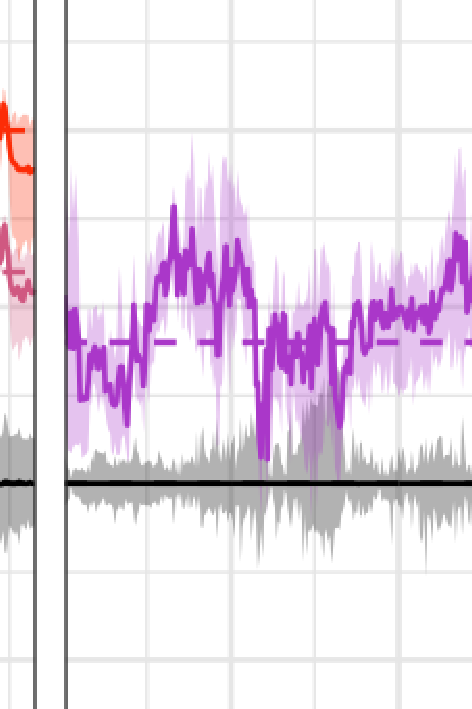
\includegraphics{/Users/aileneettinger/git/radcliffe/Analyses/figures/WarmingEffects_TimeSeries_SoilTemp1Mean_Deviation_NoPrecip.png}
 \caption{\textbf{Deviations in daily observed warming from mean soil temperature for 10 study sites,} excluding data from plots that manipulated precipitation. We show mean soil, rather than above-ground, temperature, as this was the most frequently recorded temperature variable in the C3E database. Solid lines show observed difference between warming treatment (colors) and control (black) plots, averaged across replicates and years; shading shows 95\% confidence intervals. Dashed lines represent target warming levels. Two sites not shown here did not monitor soil temperature. Experimental sites are ordered by low to high mean annual soil temperature (shown in the upper right corner of each panel).} %The number of temperature treatment levels vary from one (e.g. exp08, exp11) to nine (exp07 and exp10, which used an unreplicated regression design). Daily temperature values were obtained by averaging across years for each day of the year in each temperature treatment in each study. 
 \label{fig:effwarm}
 \end{figure}
 \begin{figure}[p]
   \centering
 \includegraphics{/Users/aileneettinger/git/radcliffe/Analyses/figures/blockyearvar.pdf}  
 \caption{\textbf{Observed warming (i.e., the difference between treatment and control plots) over space and time, for above-ground and below-ground temperatures,} excluding data from plots that manipulated precipitation. The solid line is the fitted relationship between observed and target warming and the dashed line shows when observed warming is exactly equal to target warming (1:1). See Supplemental Materials (especially Tables S4 and S5) for details.}
 \label{fig:blockyear}
 \end{figure}
 
 % EMW: Check if you included data from plots that manipulated precipitation whenever you don't say "excluding data from plots that manipulated precipitation" in a caption. 
 \begin{figure}[p]
\centering
 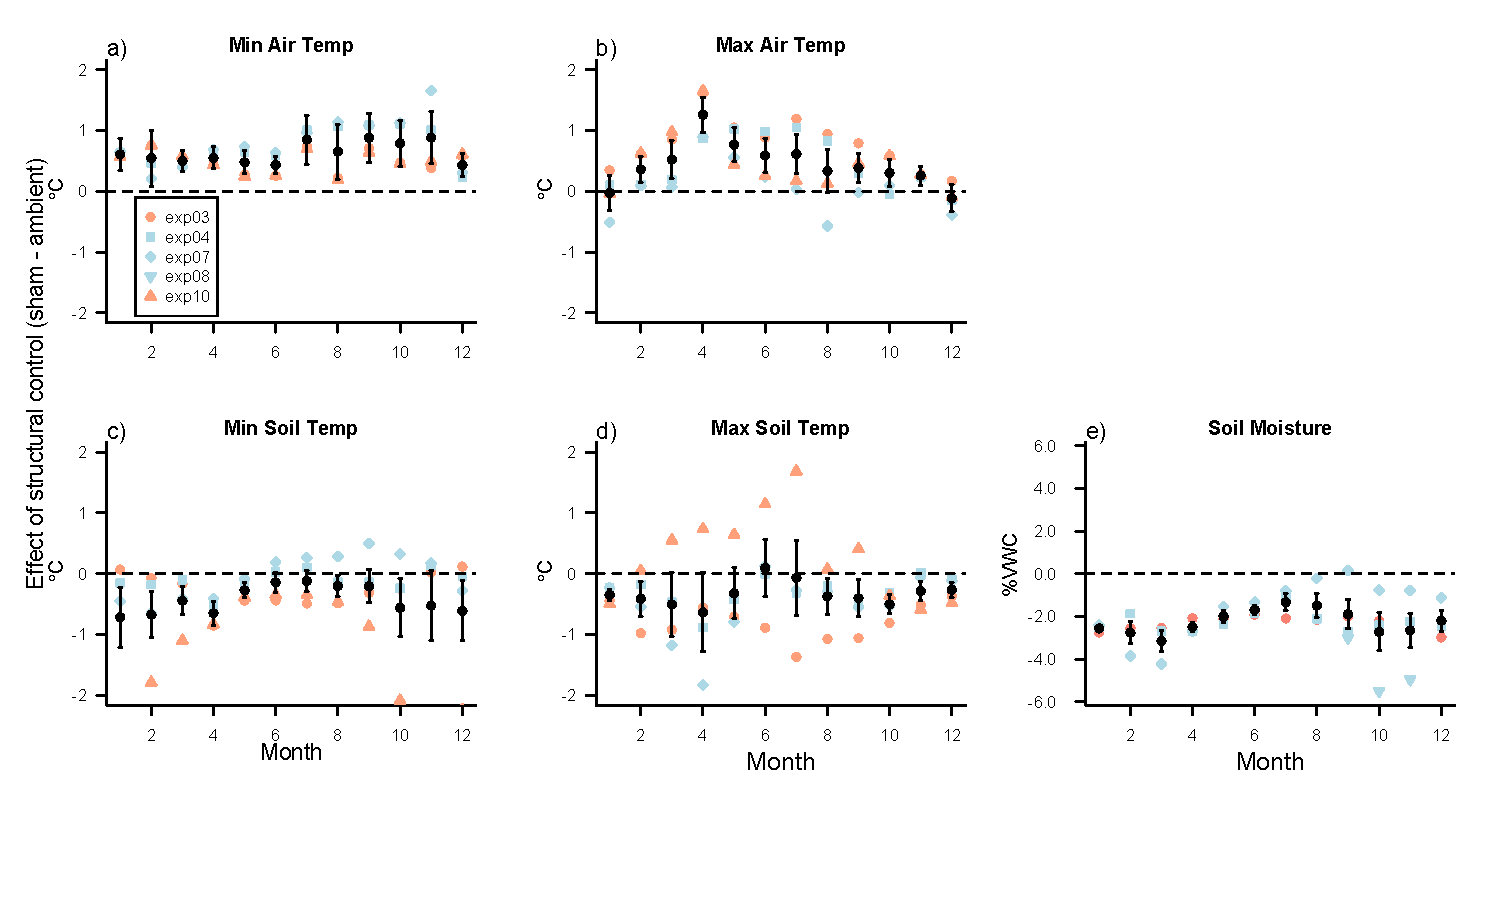
\includegraphics{/Users/aileneettinger/git/radcliffe/Analyses/figures/ShamVSAmbient_all.pdf}  
 \caption{\textbf{Deviations in measured abiotic variables by month in structural controls compared to ambient controls} (i.e., with no control chambers or warming infrastructure in place). Above-ground temperatures were higher, whereas below-ground temperature and soil moisture were lower in structural controls compared with ambient controls. We show overall (fixed) effects in black from monthly mixed-effects models; site-level random effects are shown by symbols in blue (for the three studies conducted at Harvard Forest in Massachusetts, USA) and pink (the two studies conducted at Duke Forest in North Carolina, USA).}
 \label{fig:shamamb}
 \end{figure}
\clearpage
 \begin{figure}[h]
    \centering
 \includegraphics{/Users/aileneettinger/git/radcliffe/Analyses/figures/WarmingEffects_TimeSeries_SoilMoist_Deviation_NoPrecip.png}  
 \caption{\textbf{Deviations in daily observed soil moisture,} shown for the nine study sites that continuously monitored soil moisture, excluding data from plots that manipulated precipitation. Black lines represent control plots, and colored lines represent warming treatments with various target warming levels. The number of temperature treatment levels vary from one (e.g. exp08, exp11) to nine (exp07 and exp10, which used an unreplicated regression design).  Experimental sites are ordered by low to high mean annual soil moisture (shown in the upper right corner of each plot). All experiments measured soil moisture in volumetric water content (VWC, as a proportion of the soil volume in the sample, scaled from 0 to 1)}. 
 \label{fig:mois}
 \end{figure}
 
 \begin{figure}[h]
 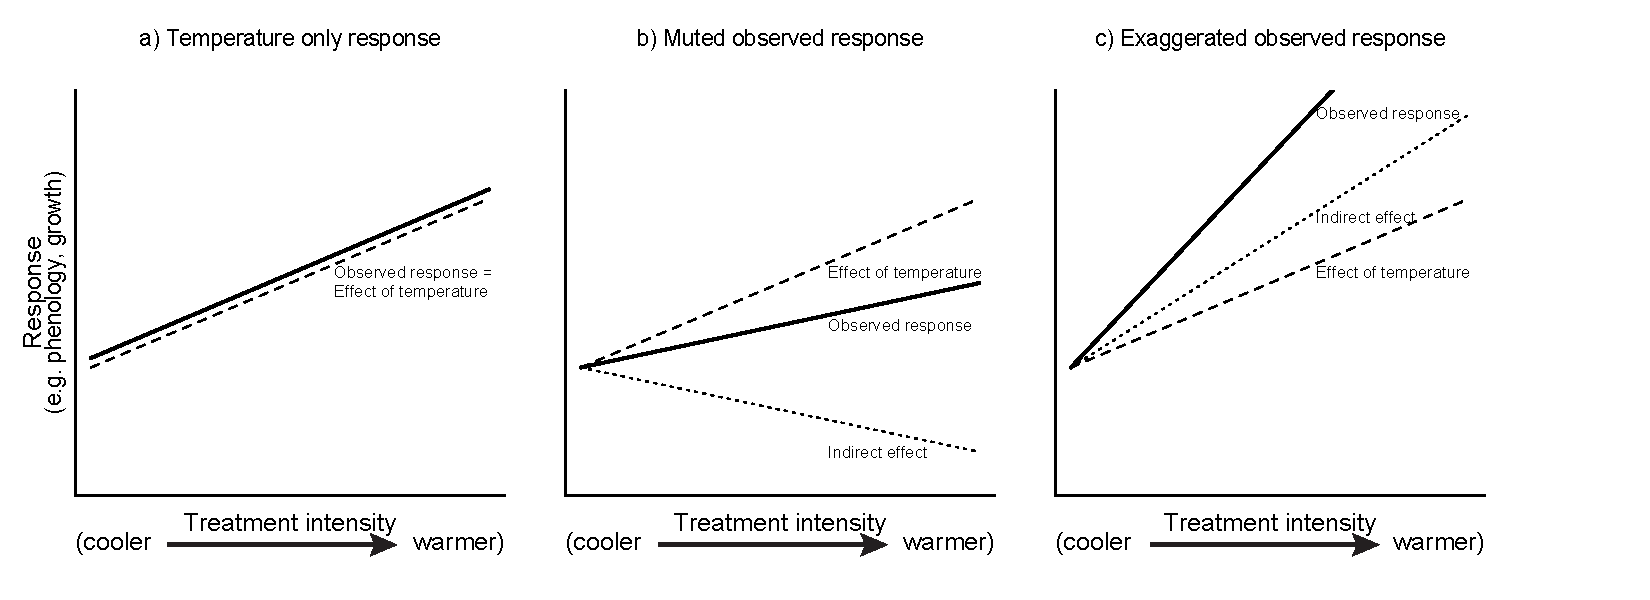
\includegraphics{/Users/aileneettinger/git/radcliffe/Analyses/figures/DirIndWarmingEffects.pdf} 
 \caption{\textbf{Theoretical biological responses to experimental climate change and their interpretation}. Direct responses to temperature alone (a) can be easily understood. Complications arise when biological responses are a mix of the direct and indirect effects of experimental warming. Then experimental warming may cause biological responses to be muted (b) or exaggerated (c). Slopes of these example lines assume a linear response with additive direct and indirect effects. The relationship between these effects could be more complex (e.g., nonlinear; antagonistic, multiplicative, or otherwise interactive).} 
\label{fig:biolimp}
\end{figure}

%CRR: can we get some sort of error around the lines here?  I like the simplicity of the figure but with no data points shown (for understandable reasons), its hard to get an idea of how precise each of those effects are.  Also, what are the units of the x-axis? degrees C?  or is it categorical?  I had a hard time when glancing through understanding which in Fig 6 vs. 7 was conceptual versus data-based.
\begin{figure}[h]
 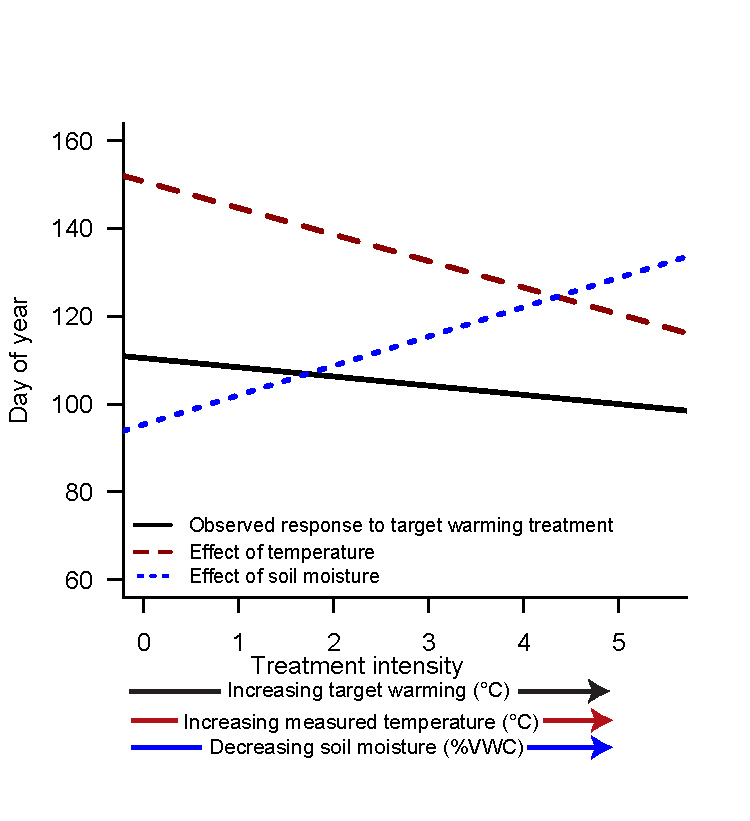
\includegraphics{/Users/aileneettinger/git/radcliffe/Analyses/figures/DirIndWarmingEffects_ExBBSM_reltemp.pdf} 
 %
 \caption{\textbf{Observed response of budburst day of year to experimental climate change} is an example of a muted response: the observed response to increasing treatment intensity (i.e., the coefficient of a model fit with only target temperature as the explanatory variable, black line; units for x-axis are \degree C of target warming) suggests a weaker temperature sensitivity than the effect of temperature in a more biologically accurate (and better-fitting) model that includes both measured above-ground temperature (dashed red line, for which x-axis units are \degree C of measured temperature)  and soil moisture (dotted blue line, for which x-axis units are \% VWC,decreasing from left to right in conjunction with warming intensity), as well as their interaction. This is because experimental warming dries out the soil in addition to increasing temperatures, and both climate variables affect the timing of budburst. Whereas increasing temperatures advance budburst, decreasing soil moisture has a delaying effect. See Supplemental Materials, especially Tables S14 \& S15, for model details.} 
 
\label{fig:phen}
\end{figure}
  
%%%%%%%%%%%%%%%%%%%%%%%%%%%%%%%%%%%%%%%%
\end{document}
%%%%%%%%%%%%%%%%%%%%%%%%%%%%%%%%%%%%%%%%
